\chapter{Verfahren}
Das Verfahren zur Schattenberechnung besteht grundsätzlich aus drei Schritten.
\begin{enumerate}
	\item Occlussionmap
			\textit{Licht Einflussbereich}
	\item Sample Distanz
			\textit{Licht weite bis zur ersten Blockade.}
	\item Render Licht
			\textit{Wie wird das Licht gerendert}
\end{enumerate}
Die verwendete Methodik ist ein Raycastverfahren das durch einige Mathematische Umformungen der Texturen den Raycast stark vereinfacht.

\section{Occlussionmap}
Zur Licht Berechnung muss zuerst eine Occlusionmap erstellt, wie in Abbildung \ref{o_1} zu sehen. Diese Textur Bildet ab welchen Bereich das Licht vom Level(Abbildung \ref{level_1}) abdeckt. 
\begin{figure}[h]
	\centering
	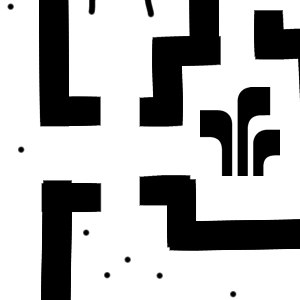
\includegraphics{images/oclusion.png}
	\caption{Occlussionmap}
	\label{o_1}
\end{figure}
\begin{figure}[h]
	\centering
	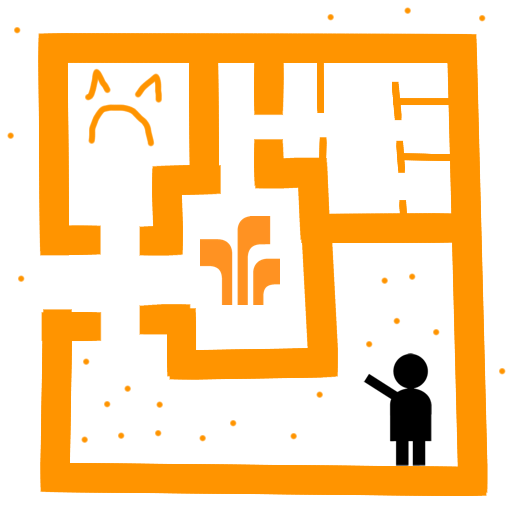
\includegraphics[scale=0.5]{images/test.png}
	\caption{Testgrafik}
	\label{level_1}
\end{figure}


\section{Sample Distanz}
Die Occlusionmap wird zur besseren Parallelisierbarkeit in Polarkoordinaten gesampelt.\ref{o_2}\\
\begin{figure}[h]
	\centering
	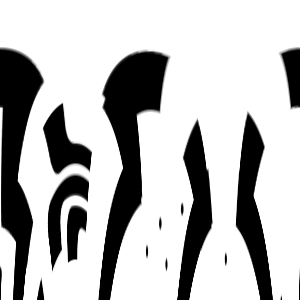
\includegraphics{images/oclusion_polar_2.png}
	\caption{Oclussionmap in polar Koordinaten}
	\label{o_2}
\end{figure}
 So können wir von der Lichtquelle aus $360^{\circ}$ im Kreis Raycasts auf der X Achse parallelisieren. Hier wird nun für jedes $X$ eine Distanz bis zum ersten blockierenden Pixel gemessen. Bildlich vorzustellen wie in Abbildung \ref{o_3}.
\begin{figure}[h]
	\centering
	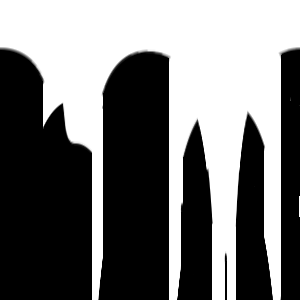
\includegraphics{images/shadow_polar_2.png}
	\caption{Symbolische Shadowmap in polar Koordinaten}
	\label{o_3}
\end{figure}
Die gemessene Distanz wird in einer 1D Textur (Abbildung \ref{o_4}) zur weiter Verarbeitung Gespeichert.
\begin{figure}[h]
	\centering
	
\includegraphics[width=0.7\textwidth,height=50px]{images/1DTexture.png}
	\caption{Gesampelte Distanzdaten.}
	\label{o_4}
\end{figure}
\section{Render Licht}
Im letzten Schritt wird ein Sprite in der Größe des Lichtes gerendert. Durch Verwendung einer Schrittfunktion wird die Distanz zum Mittelpunkt mit der maximal Entfernung die in der Textur gespeichert wurde verglichen. Wenn der gesampelte Punkt weiter weg ist als die Gemessene Entfernung liegt der Pixel im Schatten und wird schwarz gezeichnet.

Anschließend muss das Sprite noch in das Level additiv geblendet werden.\ref{level_licht_1}
\begin{figure}[h]
	\centering
	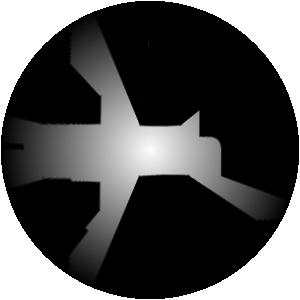
\includegraphics{images/shadow_shadow_2.png}
	\caption{Shadowmap gerendert}
	\label{shadows_1}
\end{figure}
\begin{figure}[h]
	\centering
	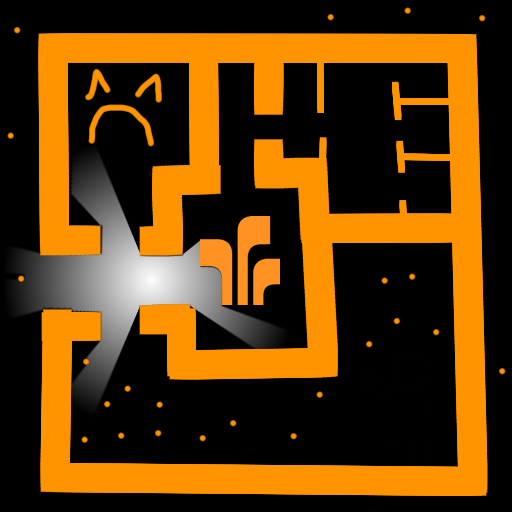
\includegraphics[scale=0.75]{images/final.png}
	\caption{Level mit einem Licht}
	\label{level_licht_1}
\end{figure}